\section{Traffic Management Optimization Using Multi-Objective Evolutionary Algorithms}

In this task, we have applyed a Multi-Objective Evolutionary Algorithm (MOEA) to optimize traffic management
strategies for selected New York City (NYC) areas, in order to  minimize conflicting
objectives, Total Travel Time (TTT) and Fuel Consumption (FC), using real-world traffic data
from NYC Open Data. The traffic management strategy has involved controlling traffic signal timings (green, yellow, and 
red light durations), and setting speed limits on these segments. We have developed an MOEA that optimized these parameters to achieve the best trade-off 
between minimizing TTT and FC.

\subsection{The Dataset, and Preprocessing}

In addition, we hvae used two datasets from the NYC Open Data portal,
1. NYC Traffic Volume Counts.
2. Traffic Speed Data.
We have focused on optimizing traffic management for the three road segments in New 
York City;  
1. 5th Ave between 42nd St and 47th St (Manhattan) 
2. Atlantic Ave between Flatbush Ave and Bedford Ave (Brooklyn) 
3. Queens Blvd between Union Tpke and Yellowstone Blvd (Queens) 

We have Identified and preprocess relevant data points, such as peak-hour traffic volumes, 
average speeds, and any available environmental indicators.

\begin{figure}[h]
    \centering
    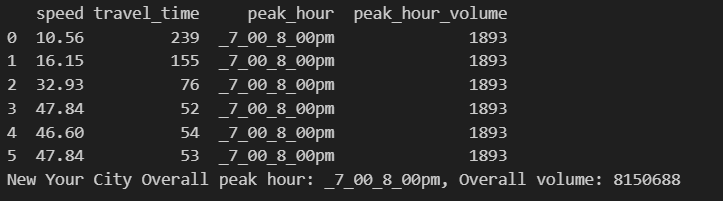
\includegraphics[width=0.5\textwidth]{figures/peak_huours.PNG}
    \caption{The peak-hour traffic}
    \label{fig:sample}
\end{figure}


Calculate the peak-hour traffic

